\section{Tecnologías}
Para el desarrollo del sistema, existen varias tecnologías en el mercado que cumplen con el propósito de desarrollar el sistema y alcanzar los objetivos planteados. Para esto es necesario tener el conocimiento acerca de las características que pueden brindar las tecnologías que se tienen al alcance y hacer una elección sobre cuales ofrecen mayores ventajas a la hora de desarrollar el sistema.
\vspace{10mm}
	\begin{table}[b!]
    \centering
    \vspace{-30mm}
      \begin{tabular}{|p{2cm}|ll}
        \hline
        
        \multicolumn{2}{|c|}{{\bf Cuadro comparativo de tecnologías}} \\ 
        \hline
          \multicolumn{1}{|p{4cm}|}{{\bf Nombre}} & 
		  \multicolumn{1}{p{10cm}|}{{\bf Características}}\\

        \hline
          \multicolumn{1}{|p{5cm}|}{Base de datos relacional} & 
          \multicolumn{2}{p{10cm}|}{\begin{itemize}
          \vspace{-5mm}
        \item Es un tipo de base de datos que cumple con el modelo relacional.
        \item Permite establecer interconexiones o relaciones entre los datos,y a través de dichas conexiones relacionar los datos de ambas tablas, de ahí proviene su nombre: \"modelo relacional\".
        \item No pueden existir dos tablas con el mismo nombre ni registro.
        \item Cada tabla es a su vez un conjunto de campos (columnas) y registros (filas).
        \item Las claves primarias son la clave principal de un registro dentro de una tabla y estas deben cumplir con la integridad de datos.\cite{28}
       
      \end{itemize}} \\
         
        \hline
          \multicolumn{1}{|p{5cm}|}{Bases de datos no relacional} & 
          \multicolumn{1}{p{10cm}|}{
          \begin{itemize}
          \vspace{-5mm}
          \item Los datos almacenados no requieren estructuras fijas como tablas, normalmente no soportan operaciones JOIN.
        \item Pueden manejar enormes cantidades de datos.
        \item No generan cuellos de botella.
        \item Escalamiento sencillo.
        \item Se ejecutan en clústers de máquinas baratas.
        \item No usan SQL como el principal lenguaje de consultas \cite{29}
      \end{itemize}} \\ 
       \hline
      \end{tabular}
    \end{table}

\newpage
	\begin{table}[b!]
    \centering
    \vspace{-5mm}
      \begin{tabular}{|p{2cm}|ll}
        \hline
          \multicolumn{1}{|p{5cm}|}{Base de datos Orientada a grafos} & 
          \multicolumn{2}{p{10cm}|}{\begin{itemize}
          \vspace{-5mm}
        \item Representa la información como nodos de un grafo y sus relaciones con las aristas del mismo
        \item Consultas más amplias y no demarcadas por tablas.
        \item No hay que definir un número determinado de atributos.
        \item Los registros también son de longitud variable, evitando tener que definir un tamaño y también posibles fallas en la base de datos.
        \item Se puede recorrer directamente la base de datos de forma jerárquica, obtener el nodo abuelo del nodo y viceversa.
        \cite{30}
      \end{itemize}} \\
       \hline
      \end{tabular}
      \caption{Tipos de bases de datos}
      \label{table: comparacion de bd}
    \end{table}
    
\newpage
	\begin{table}[b!]
    \centering
      \begin{tabular}{|p{2cm}|ll}
        \hline
        \multicolumn{2}{|c|}{{\bf Cuadro comparativo de tecnologías}} \\ 
        \hline
          \multicolumn{1}{|p{4cm}|}{{\bf Nombre}} & 
		  \multicolumn{1}{p{10cm}|}{{\bf Características}}\\
        \hline
          \multicolumn{1}{|p{5cm}|}{
\includegraphics[width=0.3\textwidth]{images/neo4j}} & 
          \multicolumn{2}{p{10cm}|}{\begin{itemize}
          \vspace{-15mm}
        \item Es una base de datos open-source desarrollada en lenguaje Java.
        \item Permite realizar transacciones ACID.
        \item Manera su propio lenguaje de query, Cypher.
        \item Puede contener billones de nodos y relaciones.
        \item Rápido recorriendo relaciones, este tipo de queries se conoce como transversals
        \item Las escrituras se pueden realizar en cualquier instancia del clúster.
        \item Proporciona una API pudiendo utilizarse en distintos lenguajes.
        \cite{31}
      \end{itemize}} \\
        \hline
          \multicolumn{1}{|p{5cm}|}{
\includegraphics[width=0.3\textwidth]{images/InfiniteGraph}} & 
          \multicolumn{1}{p{10cm}|}{
          \begin{itemize}
          \vspace{-7mm}
        \item Poseé almacenamiento en la nube.
        \item Apoyo de consultas en paralelo.
        \item Precios felixibles y opciones de licencia.
        \item Totalmente transaccional y multi-hilo.
        \cite{32}
      \end{itemize}} \\ 
        \hline
          \multicolumn{1}{|p{3cm}|}{
\includegraphics[width=0.3\textwidth]{images/InfoGrid}} & 
          \multicolumn{1}{p{10cm}|}{
          \begin{itemize}
          \vspace{-10mm}
        \item Recorrido Gráfico y consultas de tipo relacional.
        \item Indexación personalizable.
        \item Gestión de almacenamiento personalizable.\cite{33}
      \end{itemize}}\\ 
         \hline
      \end{tabular}
      \caption{Cuadro comparativo de gestores de bases de datos orientadas a grafos}
      \label{table:bd orientadas a grafos}
    \end{table}

\newpage
\begin{table}[b!]
    \centering
      \begin{tabular}{|p{1cm}|l}
        \hline
        \multicolumn{2}{|c|}{{\bf Cuadro comparativo de tecnologías}} \\ 
        \hline
          \multicolumn{1}{|p{4cm}|}{{\bf Nombre}} & 
		  \multicolumn{1}{p{10cm}|}{{\bf Características}}\\
		 \hline
          \multicolumn{1}{|p{5cm}|}{
\includegraphics[width=0.3\textwidth]{images/bootstrap}} & 
          \multicolumn{1}{p{10cm}|}{\begin{itemize} 
       \vspace{-20mm}
          \item Es un framework o conjunto de herramientas de software libre para diseño de sitios y aplicaciones web. 
        \item Contiene plantillas de diseño con tipografía, formularios, botones, cuadros, menús de navegación y otros elementos de diseño basado en HTML y CSS, así como, extensiones de JavaScript opcionales adicionales.
        \item Es compatible con la mayoría de los navegadores web.
        \item Bootstrap es de código abierto y está disponible en GitHub. 
        \item Desde la versión 2.0 también soporta diseños responsivos. Esto significa que el diseño gráfico de la página se ajusta dinámicamente, tomando en cuenta las características del dispositivo usado (Computadoras, tabletas, teléfonos móviles).
        \cite{34}
      \end{itemize}} \\
        \hline
          \multicolumn{1}{|p{5cm}|}{
\includegraphics[width=0.3\textwidth]{images/foundation}} & 
          \multicolumn{1}{p{10cm}|}{ 
          \begin{itemize}
                 \vspace{-20mm}
          \setlist[itemize]{noitemsep, topsep=0pt}  
          	\item Incluye los patrones necesarios más comunes para rápidamente maquetar un sitio responsivo
            \item A través del uso de Sass mixins, los componentes de Foundation son fácilmente estilizados y sencillos de extender.
            \item Las páginas web se ajustan a diferentes dispositivos.
            \item Open source y está disponible en GitHub.
            \cite{35}
         \end{itemize}}\\ 
        \hline
      \end{tabular}
      \caption{Cuadro de tecnologías para diseño Web}
      \label{table:Cuadro comparativo de tecnologias web}
    \end{table}

\newpage
\begin{table}[b!]
    \centering
    \vspace{-30mm}
      \begin{tabular}{|p{2cm}|ll}
        \hline
        \multicolumn{2}{|c|}{{\bf Cuadro comparativo de tecnologías}} \\ 
        \hline
          \multicolumn{1}{|p{4cm}|}{{\bf Nombre}} & 
		  \multicolumn{1}{p{10cm}|}{{\bf Características}}\\
        \hline
          \multicolumn{1}{|p{5cm}|}{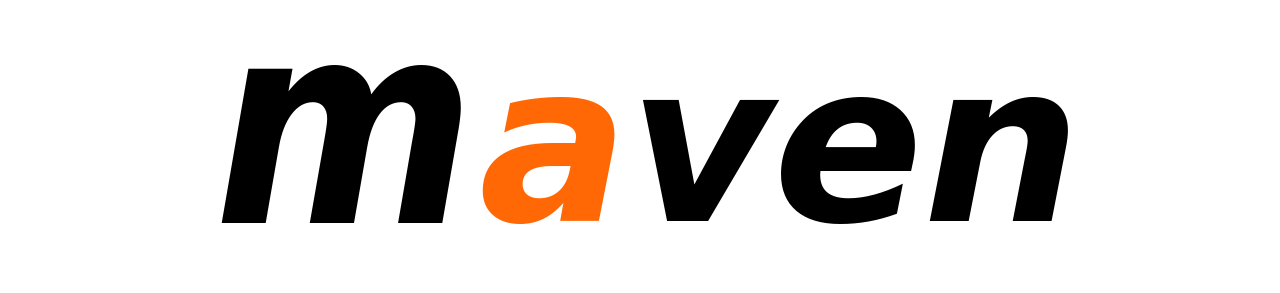
\includegraphics[width=0.3\textwidth]{images/maven}} & 
          \multicolumn{2}{p{10cm}|}{\begin{itemize}
          \vspace{-10mm}
        \item Es una herramienta de software para la gestión y construcción de proyectos.
        \item Tiene un modelo de configuración de construcción más simple, basado en un formato XML.
        \item Utiliza un Project Object Model (POM) para describir el proyecto de software a construir, sus dependencias de otros 				módulos y componentes externos, y el orden de construcción de los elementos.
        \item  Viene con objetivos predefinidos para realizar ciertas tareas claramente definidas, como la compilación del código y su 		empaquetado.
        \item El motor incluido en su núcleo puede dinámicamente descargar plugins de un repositorio.
        \item Está construido usando una arquitectura basada en plugins que permite que utilice cualquier aplicación controlable a través de la entrada estándar. 
       \cite{36}
      \end{itemize}} \\
        \hline
          \multicolumn{1}{|p{5cm}|}{
\includegraphics[width=0.3\textwidth]{images/ant}} & 
          \multicolumn{1}{p{10cm}|}{
          \begin{itemize}
          \vspace{-27mm}
          \item Es una herramienta usada en programación para la realización de tareas mecánicas y repetitivas, normalmente durante la fase de compilación y construcción (build). 
        \item Es un software para procesos de automatización de compilación, similar a Make pero desarrollado en lenguaje Java y requiere la plataforma Java, así que es más apropiado para la construcción de proyectos Java.
        \item Esta herramienta, hecha Java, tiene la ventaja de no depender de las órdenes del shell de cada sistema operativo, sino que se basa en archivos de configuración XML 
        \item  Ant utiliza XML para describir el proceso de generación y sus dependencias. \cite{37}
      \end{itemize}} \\ 
       \hline
      \end{tabular}
       \caption{ software para la gestión y construcción de proyectos}
      \label{table:Cuadro Comparativo de software para la gestión y construcción de proyectos}
    \end{table}

\newpage
\begin{table}[b!]
    \centering
    \vspace{-30mm}
      \begin{tabular}{|p{2cm}|ll}
        \hline
        \multicolumn{2}{|c|}{{\bf Cuadro comparativo de tecnologías}} \\ 
        \hline
          \multicolumn{1}{|p{4cm}|}{{\bf Nombre}} & 
		  \multicolumn{1}{p{10cm}|}{{\bf Características}}\\
        \hline
          \multicolumn{1}{|p{5cm}|}{
\includegraphics[width=0.3\textwidth]{images/git}} & 
          \multicolumn{2}{p{10cm}|}{\begin{itemize}
          \vspace{-17mm}
        \item Es un software de control de versiones open-source.
        \item Fuerte apoyo al desarrollo no lineal, por ende rapidez en la gestión de ramas y mezclado de diferentes versiones. 
        \item Git incluye herramientas específicas para navegar y visualizar un historial de desarrollo no lineal.
        \item Gestión distribuida, Git le da a cada programador una copia local del historial del desarrollo entero, y los cambios se propagan entre los repositorios locales.
         \item Los repositorios Subversion y svk se pueden usar directamente con git-svn.
        \item Gestión eficiente de proyectos grandes, dada la rapidez de gestión de diferencias entre archivos, entre otras mejoras de optimización de velocidad de ejecución.
        \item Todas las versiones previas a un cambio determinado, implican la notificación de un cambio posterior en cualquiera de ellas a ese cambio.\cite{38}
      \end{itemize}} \\
        \hline
          \multicolumn{1}{|p{5cm}|}{
\includegraphics[width=0.3\textwidth]{images/subversion}} & 
          \multicolumn{1}{p{10cm}|}{
          \begin{itemize}
          \vspace{-35mm}
          \item Es software libre bajo una licencia de tipo Apache/BSD.
        \item Utiliza el concepto de revisión para guardar los cambios producidos en el repositorio.         
        \item  Se sigue la historia de los archivos y directorios a través de copias y renombrados.
      	\item Las modificaciones (incluyendo cambios a varios archivos) son atómicas.
      	\item La creación de ramas y etiquetas es una operación más eficiente.
      	\item Se envían sólo las diferencias en ambas direcciones.
      	\item Maneja eficientemente archivos binarios.
      	\item El manejo de cambio de nombres de archivos no es completo. Lo maneja como la suma de una operación de copia y una de 	borrado. \cite{39}
      \end{itemize}} \\ 
       \hline
      \end{tabular}
      \caption{Software para el control de versiones}
      \label{table: comparacion control de versiones}
    \end{table}

\newpage
\begin{table}[b!]
    \centering
    \vspace{-30mm}
      \begin{tabular}{|p{2cm}|ll}
        \hline
        \multicolumn{2}{|c|}{{\bf Cuadro comparativo de tecnologías}} \\ 
        \hline
          \multicolumn{1}{|p{4cm}|}{{\bf Nombre}} & 
		  \multicolumn{1}{p{10cm}|}{{\bf Características}}\\
        \hline
          \multicolumn{1}{|p{5cm}|}{
\includegraphics[width=0.3\textwidth]{images/java}} & 
          \multicolumn{2}{p{10cm}|}{\begin{itemize}
          \vspace{-25mm}
        \item Es un lenguaje de programación de propósito general, concurrente, orientado a objetos 
        \item El API de programación es muy sencilla, flexible y extensible.
        \item Podemos implementar los servletsyaya que no son procesos independientes,se ejecutan dentro del mismo proceso que la JVM mejorando notablemente el rendimiento y reduciendo la carga computacional y de memoria requeridas.
		\item Las JSPs son páginas que se compilan dinámicamente de modo que el código que se consigue una ventaja en rendimiento substancial frente a muchos lenguajes interpretados.
         \item La especificación de Servlets y JSPs define un API de programación.
         \item Los requisitos para un servidor ya que se puedan desplegar estos componentes para formar aplicaciones web dinámicas completas. \cite{40}
      \end{itemize}} \\
        \hline
      \end{tabular}
      \caption{Lenguaje de desarrollo y tecnologías relacionadas}
      \label{table: Lenguaje de desarrollo}
    \end{table}

\clearpage
    \newpage
    Teniendo el conocimiento sobre las tecnologías que se tienen al alcance, la tabla~\ref{table: tecnologias usadas}se plantea utilizar las siguientes tecnologías para el desarrollo del sistema:
    \begin{table}[b!]
    \centering
    \vspace{33mm}
      \begin{tabular}{|p{2cm}|ll}
        \hline
        \multicolumn{2}{|c|}{{\bf Tecnologías a usar}} \\ 
        \hline
          \multicolumn{1}{|p{4cm}|}{{\bf Tecnología}} & 
		  \multicolumn{1}{p{10cm}|}{{\bf Ventajas}}\\
        \hline
          \multicolumn{1}{|p{5cm}|}{Bases de datos Orientadas  Grafos} & 
          \multicolumn{2}{p{10cm}|}{\begin{itemize}
          \vspace{-5mm}
         \item Debido a que están orientadas a mapear relaciones con mayor agilidad, y tienen una estructura flexible
         \item Están orientadas a consultas amplias. 
         \item Al ser orientadas a grafos brindan la posibilidad de acceder a los datos a través de algoritmos de recorrido de grafos.
         \item Están diseñadas para soportar grande volúmenes de información.
      \end{itemize}} \\
        \hline
          \multicolumn{1}{|p{5cm}|}{
\includegraphics[width=0.3\textwidth]{images/neo4j}} & 
          \multicolumn{1}{p{10cm}|}{
          \begin{itemize}
          \vspace{-15mm}
       \item A pesar de que es una base de datos NoSQL, acepta transacciones ACID.
       \item Tiene una licencia gratuita open-source.
       \item Soporta diferentes lenguajes, entre ellos Java, Python y Ruby.
       \item Es una herramienta en crecimiento que es altamente escalable.
       \item La experiencia que tienen en el campo.
      \end{itemize}} \\ 
       
        \hline
      \end{tabular}
    \end{table}
\newpage
\begin{table}[b!]
\centering
\begin{tabular}{|p{2cm}|ll}
        \hline
       \multicolumn{1}{|p{5cm}|}{
\includegraphics[width=0.3\textwidth]{images/bootstrap}}& 
          \multicolumn{1}{p{10cm}|}{
          \begin{itemize}
          \vspace{-15mm}
          \item El diseño de sitios y aplicaciones web es de licencia libre.
          \item El diseño de las  plantillas es basado en HTML y CSS.
          \item Sus diseños son responsivos, esto quiere decir que las páginas web se ajustan al dispositivo donde se este visualizando  
          \item Es compatible con la mayoría de navegadores.
          \item Las plantillas son de gran utilidad al trabajar con estilos
          \item Es una tecnología conocida por el equipo de trabajo.
      \end{itemize}} \\
\hline
 \multicolumn{1}{|p{5cm}|}{
\includegraphics[width=0.3\textwidth]{images/java}}& 
          \multicolumn{1}{p{10cm}|}{
          \begin{itemize}
          \vspace{-20mm}
          \item Nos permite hacer programación concurrente.
        \item Para el uso de servidores , Java es eficiente, desde la aparición de la especificación de Servlets y JSP.
        \item Las JSP's nos permiten la  creación de sitios web dinámicos.
        \item JSP es un lenguaje multiplataforma. Creado para ejecutarse del lado del servidor.
        \item El Código separado de la lógica del programa.
        \item Las páginas son compiladas en la primera petición.
        \item Permite separar la parte dinámica de la estática en las páginas web.
        \item Es una tecnología conocida por el equipo de trabajo.
      \end{itemize}} \\
      \hline
      \end{tabular}
    \end{table}

  \newpage
    \begin{table}[b!]
    \centering
    \vspace{33mm}
      \begin{tabular}{|p{2cm}|ll}
        \hline
        \multicolumn{2}{|c|}{{\bf Tecnologías a usar}} \\ 
        \hline
          \multicolumn{1}{|p{4cm}|}{{\bf Tecnología}} & 
		  \multicolumn{1}{p{10cm}|}{{\bf Ventajas}}\\
        \hline
          \multicolumn{1}{|p{5cm}|}{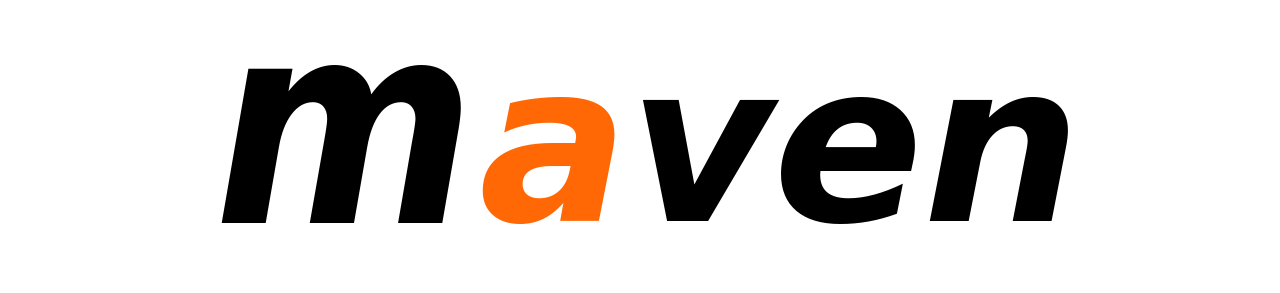
\includegraphics[width=0.3\textwidth]{images/maven}} & 
          \multicolumn{2}{p{10cm}|}{\begin{itemize}
          \vspace{-5mm}
         \item La herramienta permite gestionar y construir el proyecto de manera sencilla
         \item Permite controlar las dependencias del proyecto.
         \item Existen plugins que permiten automatizar el trabajo de construcción.
      \end{itemize}} \\
        \hline
          \multicolumn{1}{|p{5cm}|}{
\includegraphics[width=0.3\textwidth]{images/git}} & 
          \multicolumn{1}{p{10cm}|}{
          \begin{itemize}
          \vspace{-15mm}
        \item La herramienta de control de versiones es open-source.
        \item Esta disponible para cualquier sistema operativo.
		    \item Integrado con github roporciona herramientas para navegar y visualizar las versiones del proyecto, así como permitir el trabajo colaborativo.
		    \item Permite revertir cambios en los archivos cuando un archivo llegue a fallar.
        \item Es una tecnología conocida por el equipo de trabajo.
      \end{itemize}} \\ 
      
        \hline
      \end{tabular}
      \label{table: tecnologias usadas}
    \end{table}


  \newpage
    \begin{table}[b!]
    \centering
    \vspace{33mm}
      \begin{tabular}{|p{2cm}|ll}
        \hline
        \multicolumn{2}{|c|}{{\bf Tecnologías usadas front-end}} \\ 
        \hline
          \multicolumn{1}{|p{4cm}|}{{\bf Tecnología}} & 
      \multicolumn{1}{p{10cm}|}{{\bf Ventajas}}\\
        \hline
          \multicolumn{1}{|p{5cm}|}{
\includegraphics[width=0.3\textwidth]{images/angular}} & 
          \multicolumn{2}{p{10cm}|}{\begin{itemize}
          \vspace{-5mm}
          \item Es un framework JavaScript para el desarrollo de aplicaciones web del lado del cliente.
         \item Es mantenido por Google y utiliza el patrón de diseño MVC.
         Angular se compone de 4 componentes principales:
         \item Directives. Angular permite extender el HTML con nuevos
               atributos llamados directivas. 
         \item Controllers. Mantienen el control de los datos en una aplicación web. 
          \item Scope. Es el componente que enlaza la vista (HTML) con el controlador (JavaScript). Es un objeto con propiedades y métodos propios disponibles.
      \end{itemize}} \\
        
        \hline
      \end{tabular}
      \label{table: tecnologias usadas}
    \end{table}

\newpage
\begin{table}[b!]
\centering
\begin{tabular}{|p{2cm}|ll}
        \hline
          \multicolumn{1}{|p{5cm}|}{Jade}& 
          \multicolumn{1}{p{10cm}|}{
          \begin{itemize}
          \vspace{5mm}
          \item Es un motor de plantillas (template engine) de alto performance
              que permite escribir páginas HTML de forma rápida.
        \item Jade usa la identación para definir la jerarquía del DOM, de esta
              forma, no se escriben tags HTML.
        \item Podríamos decir que es un pre-procesador de código HTML, equivalente a sass, stylus o less respecto a css.
      \end{itemize}} \\
\hline
            \multicolumn{1}{|p{5cm}|}{Stylus}& 
          \multicolumn{1}{p{10cm}|}{
          \begin{itemize}
          \vspace{10mm}
          \item Es un pre-procesador de CSS que surge de la necesidad de optimizar
              las hojas de estilo.
        Las principales características de stylus son:              
        \item Paréntesis, llaves, comas, puntos y comas son opcionales.
        \item Uso de variables
        \item Uso de funciones
        \item Funciones aritméticas
      \end{itemize}} \\
      \hline
      \end{tabular}
    \end{table}

\newpage
\begin{table}[b!]
\centering
\begin{tabular}{|p{2cm}|ll}
        \hline
          \multicolumn{1}{|p{5cm}|}{Gulp}& 
          \multicolumn{1}{p{10cm}|}{
          \begin{itemize}
          \vspace{5mm}
          \item Es un build system (sistema de construcción).
        \item Permite automatizar tareas comunes de desarrollo.
        \item Reducción de código JS.
        \item Compresión de imágenes.
        \item Puede utilizar todos los modulos de npm.
        \item Permite automatizar tareas repetitivas.
        \item Se puede extender su funcionalidad con modulos de node.

      \end{itemize}} \\
\hline
            \multicolumn{1}{|p{5cm}|}{Bower}& 
          \multicolumn{1}{p{10cm}|}{
          \begin{itemize}
          \vspace{10mm}
          \item Es un gestor de paquetes para el desarrollo front-end de aplicaciones web.
          \item Depende de NodeJS y npm.
        \item Trabaja con los repositorios de git y github.
        \item La gestión de paquetes puede hacerse desde la terminal.
        \item Funciones aritméticas
      \end{itemize}} \\
      \hline
      \end{tabular}
    \end{table}

    \newpage
\begin{table}[b!]
\centering
\begin{tabular}{|p{2cm}|ll}
        \hline
          \multicolumn{1}{|p{5cm}|}{Bootstrap}& 
          \multicolumn{1}{p{10cm}|}{
          \begin{itemize}
          \vspace{5mm}
          \item Es un framework que permite crear interfaces web con CSS y JS.
        \item La particularidad de este framework es el diseño responsivo
        \item Reducción de código JS.
        \item Compresión de imágenes.
        \item Puede utilizar todos los modulos de npm.
        \item Permite automatizar tareas repetitivas.
        \item Se puede extender su funcionalidad con modulos de node.

      \end{itemize}} \\
\hline
            \multicolumn{1}{|p{5cm}|}{Bower}& 
          \multicolumn{1}{p{10cm}|}{
          \begin{itemize}
          \vspace{10mm}
          \item Es un gestor de paquetes para el desarrollo front-end de aplicaciones web.
          \item Depende de NodeJS y npm.
        \item Trabaja con los repositorios de git y github.
        \item La gestión de paquetes puede hacerse desde la terminal.
        \item Funciones aritméticas
      \end{itemize}} \\
      \hline
      \end{tabular}
    \end{table}


    \newpage
    \begin{table}[b!]
    \centering
    \vspace{10mm}  
      \begin{tabular}{|p{2cm}|ll}
        \hline
        \multicolumn{2}{|c|}{{\bf Tecnologías usadas back-end}} \\ 
        \hline
          \multicolumn{1}{|p{4cm}|}{{\bf Tecnología}} & 
      \multicolumn{1}{p{10cm}|}{{\bf Ventajas}}\\
        \hline
         \multicolumn{1}{|p{5cm}|}{Spring framework} & 
          \multicolumn{2}{p{10cm}|}{\begin{itemize}
          \vspace{-5mm}
          \item Spring es un marco de trabajo cuya finalidad es facilitar el
                desarrollo de aplicaciones Java.
         \item  Simplicidad y bajo acoplamiento: Busca ser simple. Es un
                framework robusto y configurable. Gracias a la inyección de
                dependencias logra obtener bajo acoplamiento entre las clases.
         \item  Proporciona un gran infraestructura: Gracias a los módulos
                que ofrece, permite que el desarrollador se dedique a la
                lógica de la aplicación.
         \item  Ligero: Es rápido en tiempo de ejecución y no es intrusivo a
                la hora de desarrollar
      \end{itemize}} \\
        
        \hline
         \multicolumn{1}{|p{5cm}|}{Grails}& 
          \multicolumn{1}{p{10cm}|}{
          \begin{itemize}
          \vspace{10mm}
          \item Grails es un marco de trabajo para aplicaciones web libre
                desarrollado sobre el lenguaje Groovy            
          \item Pretende ser altamente productivo siguiendo algunos paradigmas
                como convención sobre configuración o no te repitas.
         \item  proporcionando un entorno de desarrollo estandarizado y
                ocultando gran parte de los detalles de configuración al
                programador.
        \item Uso de funciones
        \item Funciones aritméticas
      \end{itemize}} \\
      \hline
      \end{tabular}
      \label{table: tecnologias usadas}
    \end{table}

\newpage
\begin{table}[b!]
\centering
\begin{tabular}{|p{2cm}|ll}
        \hline
          \multicolumn{1}{|p{5cm}|}{Maven}& 
          \multicolumn{1}{p{10cm}|}{
          \begin{itemize}
          \vspace{5mm}
          \item Es una API del lenguaje de programación Java que proporciona soporte en la creación de servicios web 
          \item Su principal funcion es  simplificar el desarrollo y despliegue de los clientes y puntos finales de los servicios web.
      \end{itemize}} \\
\hline
            \multicolumn{1}{|p{5cm}|}{Apache CFX}& 
          \multicolumn{1}{p{10cm}|}{
          \begin{itemize}
          \vspace{10mm}
           \item Es un framework de código abierto para crear servicios web.           
        \item ofrece una interfaz simple para el desarrollo de clientes y endpoints sin el uso de anotaciones.
      \end{itemize}} \\
      \hline
      \end{tabular}
    \end{table}

   

\newpage
\begin{table}[b!]
\centering
\begin{tabular}{|p{2cm}|ll}
        \hline
          \multicolumn{1}{|p{5cm}|}{Maven}& 
          \multicolumn{1}{p{10cm}|}{
          \begin{itemize}
          \vspace{5mm}
          \item Es una herramienta open-source, que permite compilar y generar ejecutables a partir del código fuente.
          \item Se encarga de gestionar y construir proyectos en Java.

      \end{itemize}} \\
\hline
            \multicolumn{1}{|p{5cm}|}{Gradle}& 
          \multicolumn{1}{p{10cm}|}{
          \begin{itemize}
          \vspace{5mm}
          \item Es una herramienta de automatización para la construcción
                de proyectos.
          \item Se apoya en Groovy y de un DSL  para trabajar con un lenguaje sencillo y para la construcción de  los proyectos en comparación con Maven.
          \item Dispone de una gran flexibilidad que permite trabajar con otros
              lenguajes y no solo Java o Groovy
      \end{itemize}} \\
      \hline
      \end{tabular}
    \end{table}

   